\section*{Attention}
\color{black}
\textit{Generate contextualised embeddings $\xi^s \in \mathbb{R}^m$ using convex combination of projected simple embeddings $x \in \mathbb{R}^e$:}

\hspace{3pt} $\xi^s = \sum_t a_{st} W x^t, \quad a_{st} \geq 0, \quad \sum_t a_{st} = 1$ with $\Xi = AXW^T$\\ 

\subsection*{Transformer Architecture \hfill $X \in \mathbb{R}^{L \times e}$}
\resizebox{\linewidth}{!}{$Q = X U_Q,\, K = X U_K,\, V = X U_V$ with $U_Q, U_K \in \mathbb{R}^{e \times d}, U_V \in \mathbb{R}^{e \times e}$}\\
\underline{Single-head:} $Attention(Q, K, V) = softmax(\tfrac{QK^T}{\sqrt{d}}) V$\\
\underline{Multihead:} $Multihead(Q,K,V) = Concat(H_1, \dots, H_h)W^O$

\hfill with $H_i= Attention(XU_Q^i, XU_K^i, X U_V^i)$ where

\hfill ${U_{\{Q,K\}}^i} \in \mathbb{R}^{n\times d_k}, U_V^i \in \mathbb{R}^{e \times d_v}, W^O \in \mathbb{R}^{hd_v\times e}$

\begin{minipage}{0.5\linewidth}
\textbf{Sinusoidal Pos. Encodings:}\\
For position $t$ and feature $k$:\\ $p_{tk}=\begin{cases} \sin(t\omega_k) \quad k \text{ even} \\ \cos(t\omega_k) \quad k \text{ odd} \end{cases}\\ \hfill \text{where } \omega_k=C^{k/n}, C=10000$\\

\textbf{Self-Attention:}
$Q,K,V$ from same sequence\\

\textbf{Cross-Attention:}
$Q$ from decoder, $K,V$ from encoder\\

\textbf{Masked Attention:}
Causal mask prevents peeking
\end{minipage}
\begin{minipage}{0.5\linewidth}
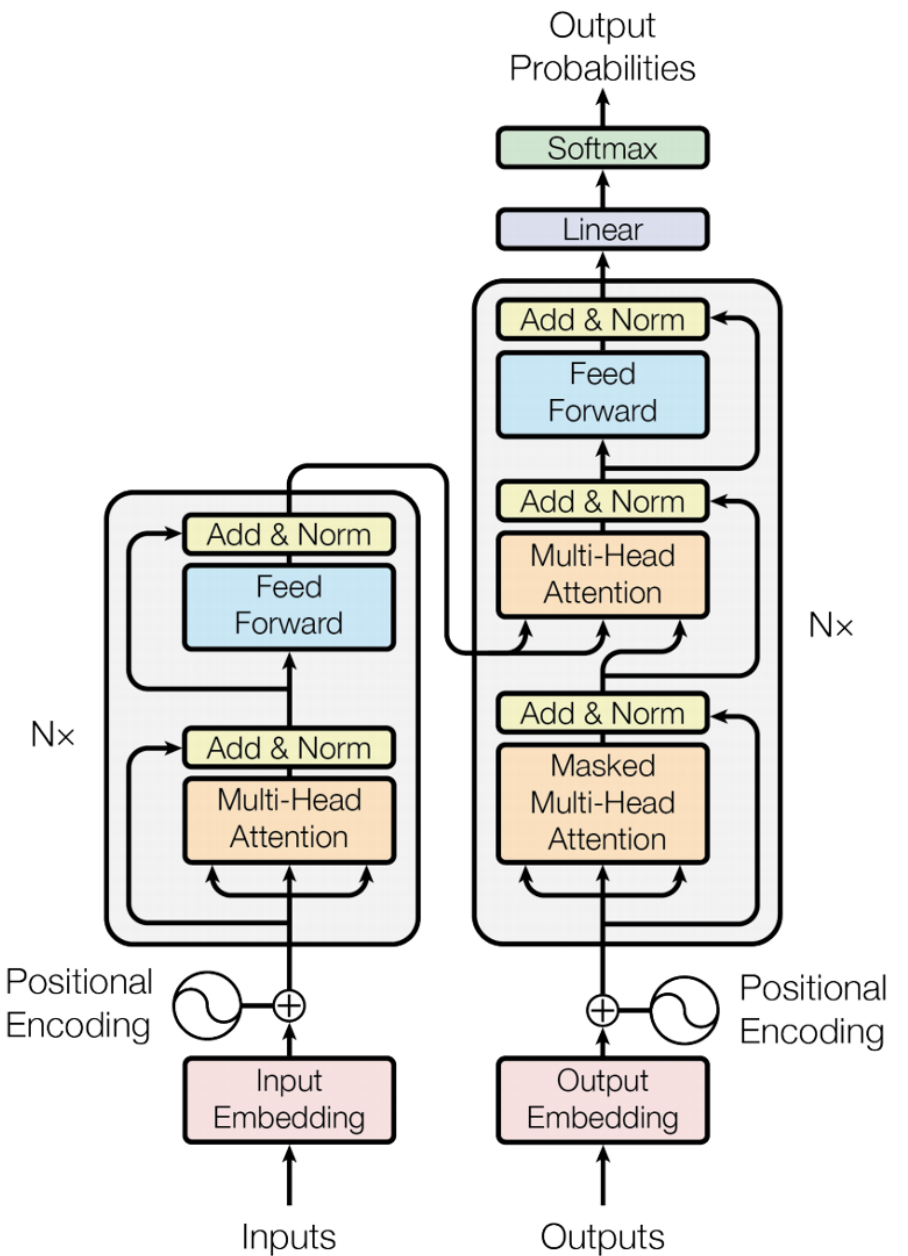
\includegraphics[angle=0, width=\linewidth]{transformer.png}\\
\end{minipage}

\textbf{RNN:} intelligent forgetting (compression)

\textbf{Transformer:} store and index intelligently\\


\subsection*{Memory Networks}
\textit{Recurrent attention model over external memory.}\\
\textbf{Recursive Associative Recall:} Given query $\mathbf q$ (e.g. question), find best matching memory cell $i$ and use its content $\mathbf m_i$ and $\mathbf q$ to generate new query - repeat
\subsection*{Applications in NLP}
\textbf{SpeechToText:} Easier to model $\mathbb P(speech | text)$ and use LLM for $\mathbb P(text)$ in $\mathbb P(text|speech) \propto \mathbb P(speech | text) \mathbb P(text)$.

\textit{Construct word embeddings that reflect the context}\\
\textbf{ELMo}: Contextualised word embeddings by stacking single CNN with bidirectional LSTMs. The contextualised embedding is derived from a parametrized convex combination of the hidden states across layers.\\
\textbf{BERT}: Bidirectional masked LLM. Pretrained by cloze task, i.e. predict masked word in text (word $\gets$ [MASK], random, or word), and by next sentence prediction, with input format \underline{[CLS], sentence A, [SEP], sentence B}. BERT is often fine-tuned for specific downstream task.\\
\textbf{GPT-n}: (Autogressive decoder model) Few, one, or zero shot learning (no gradient updates) - add task description \& examples to working memory and predict.\\
\textbf{Vision transformers}: Use vectorised image patches as ''word'' embeddings for Transformer (encoder).
\color{red}
